\chapter{Experiments}
To show the usefulness of our improvements of the automatic generator, we have compared several solvers of some minimal problems using different methods. We have used the benchmark tool of the automatic generator to generate the solvers and to compare the results.

We have divided the experiments into three parts. In each part, we are comparing easily comparable methods on which the speed up of the new implemented methods can be straightforwardly seen. In the first section, we are comparing one elimination solvers against multiple elimination solvers. In the second part, we are comparing solvers without the matrix partitioning to solvers with matrix partitioning used in the~last elimination only and to solvers with matrix partitioning used in all eliminations. In the~last section, we are comparing solvers with different strategies of~polynomial generation. One solver is generated by the systematical generator while the second one is generated using the $F_4$ strategy.

To be able to compare the solvers, we have measured the time of computing the~solutions for each set of parameters for each solver. In the tables below, we have picked up the maximal and minimal values and medians of the times for each solver. We also show the sizes of matrices to eliminate and approximate numbers of operations for each solver. By the number of operations we mean the number of operations which are needed to obtain the solutions from the set of parameters including the operations of the Gauss-Jordan eliminations. To eliminate a matrix of dimensions $m \times n$, we need to do $(\max\{m, n\})^3$ operations which is the upper bound of the time complexity of the~Gauss-Jordan elimination. To be able to compare the numerical stability of the solvers, we have substituted each computed solution back into the given equations and wrote down the results as errors. We have removed the errors equal to zero and computed the $\log_{10}$ of absolute values of errors. We have presented these values as histograms for each solver.

We have choosen the 9-point relative pose different radial distortion problem \cite{9pt} for the testing. This problem consists of four polynomial equations in four unknowns. The~number of all parameters is 63. The definition of this minimal problem can be found under the name \texttt{ku9pt} in the folder \texttt{minimalProblems} in the automatic generator. To generate the solvers, we have used the default settings of the automatic generator obtained by calling the function \textit{gbs\_InitConfig} if we do not specify differently in the~description of each experiment. We have tested the generated solvers on randomly generated data which remained the same within each experiment. Each solver was tried on $1\,000$ instances of parameters. All test were performed on Intel Xeon E5-2630 2.30~GHz based computer. The MATLAB R2014a 64-bit was used to run the~tests.

\section{Multiple elimination solver}
\label{exp:elim}
In this part, we are comparing one elimination solver to multiple elimination solvers. We have generated one solver according to the description in the section \ref{subsec:polynomialGenerator}. This first solver consist only of one elimination in the end. The second and the third solvers have been generated as explained in the section \ref{subsec:multipleSolver}. The second solver has been generated with the variable $step$ set to 1, and therefore an elimination is performed always when the maximal total degree of the generated polynomials is increased by 1. This second solver consist of four Gauss-Jordan eliminations. The third solver has been generated with the variable $step$ set to 2. This means, that an elimination is performed when the maximal total degree of the generated polynomials is increased by 2. This solver consists of two eliminations.

We have used the benchmark templates specified in the function \textit{bench\_elimination} in the folder \texttt{benchmark} in the automatic generator. All other settings remained set to default values.

The computation times, sizes of matrices to eliminate and numbers of operations required by these solvers are shown in the Table \ref{tab:elim}. The numerical stability of the~solvers is shown in the Figure \ref{graph:elim} as histogram of $\log_{10}$ of absolute values of errors.

\begin{figure}[ht]
  \centering
  \resizebox{0.95\textwidth}{!}{% GNUPLOT: LaTeX picture with Postscript
\begingroup
  \makeatletter
  \providecommand\color[2][]{%
    \GenericError{(gnuplot) \space\space\space\@spaces}{%
      Package color not loaded in conjunction with
      terminal option `colourtext'%
    }{See the gnuplot documentation for explanation.%
    }{Either use 'blacktext' in gnuplot or load the package
      color.sty in LaTeX.}%
    \renewcommand\color[2][]{}%
  }%
  \providecommand\includegraphics[2][]{%
    \GenericError{(gnuplot) \space\space\space\@spaces}{%
      Package graphicx or graphics not loaded%
    }{See the gnuplot documentation for explanation.%
    }{The gnuplot epslatex terminal needs graphicx.sty or graphics.sty.}%
    \renewcommand\includegraphics[2][]{}%
  }%
  \providecommand\rotatebox[2]{#2}%
  \@ifundefined{ifGPcolor}{%
    \newif\ifGPcolor
    \GPcolorfalse
  }{}%
  \@ifundefined{ifGPblacktext}{%
    \newif\ifGPblacktext
    \GPblacktexttrue
  }{}%
  % define a \g@addto@macro without @ in the name:
  \let\gplgaddtomacro\g@addto@macro
  % define empty templates for all commands taking text:
  \gdef\gplbacktext{}%
  \gdef\gplfronttext{}%
  \makeatother
  \ifGPblacktext
    % no textcolor at all
    \def\colorrgb#1{}%
    \def\colorgray#1{}%
  \else
    % gray or color?
    \ifGPcolor
      \def\colorrgb#1{\color[rgb]{#1}}%
      \def\colorgray#1{\color[gray]{#1}}%
      \expandafter\def\csname LTw\endcsname{\color{white}}%
      \expandafter\def\csname LTb\endcsname{\color{black}}%
      \expandafter\def\csname LTa\endcsname{\color{black}}%
      \expandafter\def\csname LT0\endcsname{\color[rgb]{1,0,0}}%
      \expandafter\def\csname LT1\endcsname{\color[rgb]{0,1,0}}%
      \expandafter\def\csname LT2\endcsname{\color[rgb]{0,0,1}}%
      \expandafter\def\csname LT3\endcsname{\color[rgb]{1,0,1}}%
      \expandafter\def\csname LT4\endcsname{\color[rgb]{0,1,1}}%
      \expandafter\def\csname LT5\endcsname{\color[rgb]{1,1,0}}%
      \expandafter\def\csname LT6\endcsname{\color[rgb]{0,0,0}}%
      \expandafter\def\csname LT7\endcsname{\color[rgb]{1,0.3,0}}%
      \expandafter\def\csname LT8\endcsname{\color[rgb]{0.5,0.5,0.5}}%
    \else
      % gray
      \def\colorrgb#1{\color{black}}%
      \def\colorgray#1{\color[gray]{#1}}%
      \expandafter\def\csname LTw\endcsname{\color{white}}%
      \expandafter\def\csname LTb\endcsname{\color{black}}%
      \expandafter\def\csname LTa\endcsname{\color{black}}%
      \expandafter\def\csname LT0\endcsname{\color{black}}%
      \expandafter\def\csname LT1\endcsname{\color{black}}%
      \expandafter\def\csname LT2\endcsname{\color{black}}%
      \expandafter\def\csname LT3\endcsname{\color{black}}%
      \expandafter\def\csname LT4\endcsname{\color{black}}%
      \expandafter\def\csname LT5\endcsname{\color{black}}%
      \expandafter\def\csname LT6\endcsname{\color{black}}%
      \expandafter\def\csname LT7\endcsname{\color{black}}%
      \expandafter\def\csname LT8\endcsname{\color{black}}%
    \fi
  \fi
  \setlength{\unitlength}{0.0500bp}%
  \begin{picture}(8640.00,5040.00)%
    \gplgaddtomacro\gplbacktext{%
      \csname LTb\endcsname%
      \put(814,704){\makebox(0,0)[r]{\strut{} 0}}%
      \csname LTb\endcsname%
      \put(814,1286){\makebox(0,0)[r]{\strut{} 2}}%
      \csname LTb\endcsname%
      \put(814,1867){\makebox(0,0)[r]{\strut{} 4}}%
      \csname LTb\endcsname%
      \put(814,2449){\makebox(0,0)[r]{\strut{} 6}}%
      \csname LTb\endcsname%
      \put(814,3030){\makebox(0,0)[r]{\strut{} 8}}%
      \csname LTb\endcsname%
      \put(814,3612){\makebox(0,0)[r]{\strut{} 10}}%
      \csname LTb\endcsname%
      \put(814,4193){\makebox(0,0)[r]{\strut{} 12}}%
      \csname LTb\endcsname%
      \put(814,4775){\makebox(0,0)[r]{\strut{} 14}}%
      \csname LTb\endcsname%
      \put(946,484){\makebox(0,0){\strut{}-14}}%
      \csname LTb\endcsname%
      \put(1676,484){\makebox(0,0){\strut{}-12}}%
      \csname LTb\endcsname%
      \put(2405,484){\makebox(0,0){\strut{}-10}}%
      \csname LTb\endcsname%
      \put(3135,484){\makebox(0,0){\strut{}-8}}%
      \csname LTb\endcsname%
      \put(3865,484){\makebox(0,0){\strut{}-6}}%
      \csname LTb\endcsname%
      \put(4595,484){\makebox(0,0){\strut{}-4}}%
      \csname LTb\endcsname%
      \put(5324,484){\makebox(0,0){\strut{}-2}}%
      \csname LTb\endcsname%
      \put(6054,484){\makebox(0,0){\strut{} 0}}%
      \csname LTb\endcsname%
      \put(6784,484){\makebox(0,0){\strut{} 2}}%
      \csname LTb\endcsname%
      \put(7513,484){\makebox(0,0){\strut{} 4}}%
      \csname LTb\endcsname%
      \put(8243,484){\makebox(0,0){\strut{} 6}}%
      \put(176,2739){\rotatebox{-270}{\makebox(0,0){\strut{}Frequency}}}%
      \put(4594,154){\makebox(0,0){\strut{}log$_{10}$($|$error$|$)}}%
      \put(4594,4665){\makebox(0,0){\strut{}}}%
    }%
    \gplgaddtomacro\gplfronttext{%
      \csname LTb\endcsname%
      \put(7256,4602){\makebox(0,0)[r]{\strut{}Without matrix partitioning}}%
      \csname LTb\endcsname%
      \put(7256,4382){\makebox(0,0)[r]{\strut{}Last elimination with matrix partitioning}}%
      \csname LTb\endcsname%
      \put(7256,4162){\makebox(0,0)[r]{\strut{}All eliminations with matrix partitioning}}%
    }%
    \gplbacktext
    \put(0,0){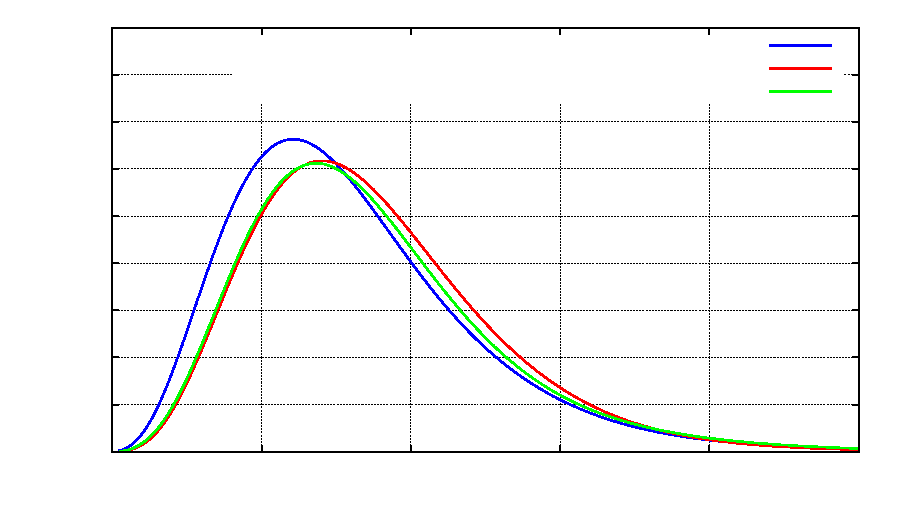
\includegraphics{graphs/elim}}%
    \gplfronttext
  \end{picture}%
\endgroup
}
  \caption{Histogram of $\log_{10}$ of absolute values of errors for one elimination and multiple elimination solvers.}
  \label{graph:elim}
\end{figure}

You can see that the numerical stability of the multiple elimination solvers is slightly worse than the numerical stability of the one elimination solver. In the contrary, the~multiple elimination solvers are approximately 1.5 times faster than the one elimination solver. Interesting is that the second and third solvers are equivalently fast, but one of them consists of four eliminations and the second one only of two eliminations. Therefore, we can not say that more eliminations lead to faster solvers. So, it is important to run benchmarks to find the optimal number of eliminations for each minimal problem and then choose the best solver for the application at hand.

\section{Matrix partitioning}
\label{exp:part}
In this section, we compare solvers using matrix partitioning, as described in the~section~\ref{subsec:matrixPart}, on multiple elimination solvers as described in the~section~\ref{subsec:multipleSolver}. We have set the variable $step$ to one so the generated solvers consist of four eliminations. The first solver has been generated without matrix partitioning. In the second one, matrix partitioning was used in the last elimination only and the third solver has been generated with matrix partitioning in all four eliminations.

The benchmark templates used for this comparison are specified in the function \textit{bench\_\-mat\-rix\-Partitioning} in the folder \texttt{benchmark} in the automatic generator. The~variable $step$ was set to 1 and all other settings remained set to default values.

The computation times, sizes of matrices to eliminate and numbers of operations required by these tree solvers are in the Table \ref{tab:part} and the numerical stability is shown as histogram of $\log_{10}$ of absolute values of errors in the Figure \ref{graph:part}.

\begin{figure}[ht]
  \centering
  \resizebox{0.95\textwidth}{!}{% GNUPLOT: LaTeX picture with Postscript
\begingroup
  \makeatletter
  \providecommand\color[2][]{%
    \GenericError{(gnuplot) \space\space\space\@spaces}{%
      Package color not loaded in conjunction with
      terminal option `colourtext'%
    }{See the gnuplot documentation for explanation.%
    }{Either use 'blacktext' in gnuplot or load the package
      color.sty in LaTeX.}%
    \renewcommand\color[2][]{}%
  }%
  \providecommand\includegraphics[2][]{%
    \GenericError{(gnuplot) \space\space\space\@spaces}{%
      Package graphicx or graphics not loaded%
    }{See the gnuplot documentation for explanation.%
    }{The gnuplot epslatex terminal needs graphicx.sty or graphics.sty.}%
    \renewcommand\includegraphics[2][]{}%
  }%
  \providecommand\rotatebox[2]{#2}%
  \@ifundefined{ifGPcolor}{%
    \newif\ifGPcolor
    \GPcolorfalse
  }{}%
  \@ifundefined{ifGPblacktext}{%
    \newif\ifGPblacktext
    \GPblacktexttrue
  }{}%
  % define a \g@addto@macro without @ in the name:
  \let\gplgaddtomacro\g@addto@macro
  % define empty templates for all commands taking text:
  \gdef\gplbacktext{}%
  \gdef\gplfronttext{}%
  \makeatother
  \ifGPblacktext
    % no textcolor at all
    \def\colorrgb#1{}%
    \def\colorgray#1{}%
  \else
    % gray or color?
    \ifGPcolor
      \def\colorrgb#1{\color[rgb]{#1}}%
      \def\colorgray#1{\color[gray]{#1}}%
      \expandafter\def\csname LTw\endcsname{\color{white}}%
      \expandafter\def\csname LTb\endcsname{\color{black}}%
      \expandafter\def\csname LTa\endcsname{\color{black}}%
      \expandafter\def\csname LT0\endcsname{\color[rgb]{1,0,0}}%
      \expandafter\def\csname LT1\endcsname{\color[rgb]{0,1,0}}%
      \expandafter\def\csname LT2\endcsname{\color[rgb]{0,0,1}}%
      \expandafter\def\csname LT3\endcsname{\color[rgb]{1,0,1}}%
      \expandafter\def\csname LT4\endcsname{\color[rgb]{0,1,1}}%
      \expandafter\def\csname LT5\endcsname{\color[rgb]{1,1,0}}%
      \expandafter\def\csname LT6\endcsname{\color[rgb]{0,0,0}}%
      \expandafter\def\csname LT7\endcsname{\color[rgb]{1,0.3,0}}%
      \expandafter\def\csname LT8\endcsname{\color[rgb]{0.5,0.5,0.5}}%
    \else
      % gray
      \def\colorrgb#1{\color{black}}%
      \def\colorgray#1{\color[gray]{#1}}%
      \expandafter\def\csname LTw\endcsname{\color{white}}%
      \expandafter\def\csname LTb\endcsname{\color{black}}%
      \expandafter\def\csname LTa\endcsname{\color{black}}%
      \expandafter\def\csname LT0\endcsname{\color{black}}%
      \expandafter\def\csname LT1\endcsname{\color{black}}%
      \expandafter\def\csname LT2\endcsname{\color{black}}%
      \expandafter\def\csname LT3\endcsname{\color{black}}%
      \expandafter\def\csname LT4\endcsname{\color{black}}%
      \expandafter\def\csname LT5\endcsname{\color{black}}%
      \expandafter\def\csname LT6\endcsname{\color{black}}%
      \expandafter\def\csname LT7\endcsname{\color{black}}%
      \expandafter\def\csname LT8\endcsname{\color{black}}%
    \fi
  \fi
  \setlength{\unitlength}{0.0500bp}%
  \begin{picture}(8640.00,5040.00)%
    \gplgaddtomacro\gplbacktext{%
      \csname LTb\endcsname%
      \put(946,704){\makebox(0,0)[r]{\strut{} 0}}%
      \csname LTb\endcsname%
      \put(946,1156){\makebox(0,0)[r]{\strut{} 50}}%
      \csname LTb\endcsname%
      \put(946,1609){\makebox(0,0)[r]{\strut{} 100}}%
      \csname LTb\endcsname%
      \put(946,2061){\makebox(0,0)[r]{\strut{} 150}}%
      \csname LTb\endcsname%
      \put(946,2513){\makebox(0,0)[r]{\strut{} 200}}%
      \csname LTb\endcsname%
      \put(946,2966){\makebox(0,0)[r]{\strut{} 250}}%
      \csname LTb\endcsname%
      \put(946,3418){\makebox(0,0)[r]{\strut{} 300}}%
      \csname LTb\endcsname%
      \put(946,3870){\makebox(0,0)[r]{\strut{} 350}}%
      \csname LTb\endcsname%
      \put(946,4323){\makebox(0,0)[r]{\strut{} 400}}%
      \csname LTb\endcsname%
      \put(946,4775){\makebox(0,0)[r]{\strut{} 450}}%
      \csname LTb\endcsname%
      \put(1078,484){\makebox(0,0){\strut{}-15}}%
      \csname LTb\endcsname%
      \put(2511,484){\makebox(0,0){\strut{}-10}}%
      \csname LTb\endcsname%
      \put(3944,484){\makebox(0,0){\strut{}-5}}%
      \csname LTb\endcsname%
      \put(5377,484){\makebox(0,0){\strut{} 0}}%
      \csname LTb\endcsname%
      \put(6810,484){\makebox(0,0){\strut{} 5}}%
      \csname LTb\endcsname%
      \put(8243,484){\makebox(0,0){\strut{} 10}}%
      \put(176,2739){\rotatebox{-270}{\makebox(0,0){\strut{}Frequency}}}%
      \put(4660,154){\makebox(0,0){\strut{}log$_{10}\Big(\big|$error$\big|\Big)$}}%
      \put(4660,4665){\makebox(0,0){\strut{}}}%
    }%
    \gplgaddtomacro\gplfronttext{%
      \csname LTb\endcsname%
      \put(7256,4602){\makebox(0,0)[r]{\strut{}Without matrix partitioning}}%
      \csname LTb\endcsname%
      \put(7256,4382){\makebox(0,0)[r]{\strut{}Last elimination with matrix partitioning}}%
      \csname LTb\endcsname%
      \put(7256,4162){\makebox(0,0)[r]{\strut{}All eliminations with matrix partitioning}}%
    }%
    \gplbacktext
    \put(0,0){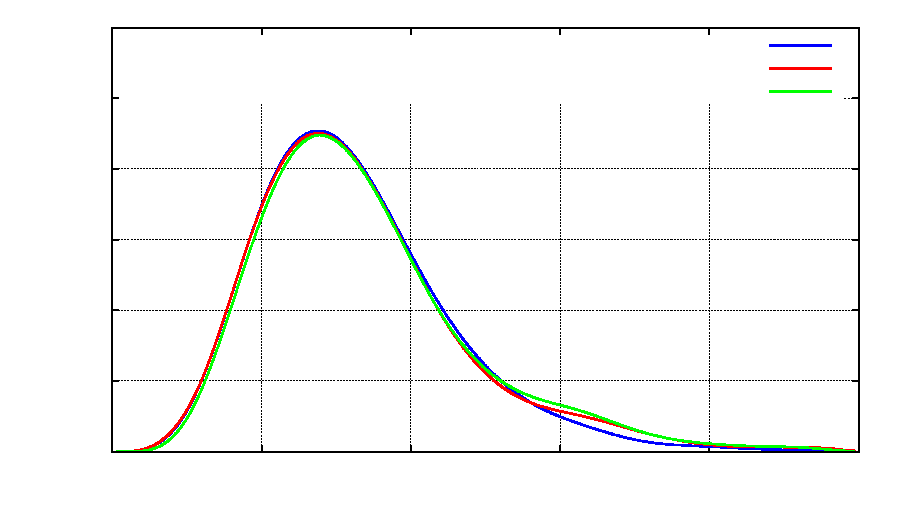
\includegraphics{graphs/part}}%
    \gplfronttext
  \end{picture}%
\endgroup
}
  \caption{Histogram of $\log_{10}$ of absolute values of errors for solver without matrix partitioning, for solver with matrix partitioning in the last elimination only and for solver with matrix partitioning in all eliminations.}
  \label{graph:part}
\end{figure}

We can see that the numerical stability remained practically the same for all three solvers. The solver with matrix partitioning in the last elimination is approximately twice faster than the solver without matrix paritioning. There is no big difference between the solver with matrix partitioning in the last elimination and the solver with matrix partitioning in all eliminations in the solver. The reason is, that when eliminating any other than the last matrix in the solver, we have to eliminate all the coupling columns. We do not have to do this when it is the last elimination. Therefore, the~speed up of the elimination of other than the last matrix is smaller than the speed up of the~last elimination.

\section{$F_4$ strategy}
\label{exp:gen}
At last, we have compared a solver generated by the systematical polynomial generator with a solver generated with the $F_4$ strategy. The first solver has been generated according to the decription in the section \ref{subsec:polynomialGenerator} using the systematical polynomial generator. The second one used the $F_4$ strategy described in the section \ref{subsec:F4}.

We have used the benchmark templates that are defined in the function \textit{bench\_poly\-nomialGenerator}, which is stored in the folder \texttt{benchmark} in the automatic generator. All other settings remained set to default values.

The numerical stabilities of both solvers are compared in the Figure \ref{graph:gen} as histogram of $\log_{10}$ of absolute values of errors. The computation times, sizes of matrices to eliminate and numbers of operations required by these solvers are in the Table \ref{tab:gen}.

\begin{figure}[ht]
  \centering
  \resizebox{0.95\textwidth}{!}{% GNUPLOT: LaTeX picture with Postscript
\begingroup
  \makeatletter
  \providecommand\color[2][]{%
    \GenericError{(gnuplot) \space\space\space\@spaces}{%
      Package color not loaded in conjunction with
      terminal option `colourtext'%
    }{See the gnuplot documentation for explanation.%
    }{Either use 'blacktext' in gnuplot or load the package
      color.sty in LaTeX.}%
    \renewcommand\color[2][]{}%
  }%
  \providecommand\includegraphics[2][]{%
    \GenericError{(gnuplot) \space\space\space\@spaces}{%
      Package graphicx or graphics not loaded%
    }{See the gnuplot documentation for explanation.%
    }{The gnuplot epslatex terminal needs graphicx.sty or graphics.sty.}%
    \renewcommand\includegraphics[2][]{}%
  }%
  \providecommand\rotatebox[2]{#2}%
  \@ifundefined{ifGPcolor}{%
    \newif\ifGPcolor
    \GPcolorfalse
  }{}%
  \@ifundefined{ifGPblacktext}{%
    \newif\ifGPblacktext
    \GPblacktexttrue
  }{}%
  % define a \g@addto@macro without @ in the name:
  \let\gplgaddtomacro\g@addto@macro
  % define empty templates for all commands taking text:
  \gdef\gplbacktext{}%
  \gdef\gplfronttext{}%
  \makeatother
  \ifGPblacktext
    % no textcolor at all
    \def\colorrgb#1{}%
    \def\colorgray#1{}%
  \else
    % gray or color?
    \ifGPcolor
      \def\colorrgb#1{\color[rgb]{#1}}%
      \def\colorgray#1{\color[gray]{#1}}%
      \expandafter\def\csname LTw\endcsname{\color{white}}%
      \expandafter\def\csname LTb\endcsname{\color{black}}%
      \expandafter\def\csname LTa\endcsname{\color{black}}%
      \expandafter\def\csname LT0\endcsname{\color[rgb]{1,0,0}}%
      \expandafter\def\csname LT1\endcsname{\color[rgb]{0,1,0}}%
      \expandafter\def\csname LT2\endcsname{\color[rgb]{0,0,1}}%
      \expandafter\def\csname LT3\endcsname{\color[rgb]{1,0,1}}%
      \expandafter\def\csname LT4\endcsname{\color[rgb]{0,1,1}}%
      \expandafter\def\csname LT5\endcsname{\color[rgb]{1,1,0}}%
      \expandafter\def\csname LT6\endcsname{\color[rgb]{0,0,0}}%
      \expandafter\def\csname LT7\endcsname{\color[rgb]{1,0.3,0}}%
      \expandafter\def\csname LT8\endcsname{\color[rgb]{0.5,0.5,0.5}}%
    \else
      % gray
      \def\colorrgb#1{\color{black}}%
      \def\colorgray#1{\color[gray]{#1}}%
      \expandafter\def\csname LTw\endcsname{\color{white}}%
      \expandafter\def\csname LTb\endcsname{\color{black}}%
      \expandafter\def\csname LTa\endcsname{\color{black}}%
      \expandafter\def\csname LT0\endcsname{\color{black}}%
      \expandafter\def\csname LT1\endcsname{\color{black}}%
      \expandafter\def\csname LT2\endcsname{\color{black}}%
      \expandafter\def\csname LT3\endcsname{\color{black}}%
      \expandafter\def\csname LT4\endcsname{\color{black}}%
      \expandafter\def\csname LT5\endcsname{\color{black}}%
      \expandafter\def\csname LT6\endcsname{\color{black}}%
      \expandafter\def\csname LT7\endcsname{\color{black}}%
      \expandafter\def\csname LT8\endcsname{\color{black}}%
    \fi
  \fi
  \setlength{\unitlength}{0.0500bp}%
  \begin{picture}(8640.00,5040.00)%
    \gplgaddtomacro\gplbacktext{%
      \csname LTb\endcsname%
      \put(946,704){\makebox(0,0)[r]{\strut{} 0}}%
      \csname LTb\endcsname%
      \put(946,1156){\makebox(0,0)[r]{\strut{} 100}}%
      \csname LTb\endcsname%
      \put(946,1609){\makebox(0,0)[r]{\strut{} 200}}%
      \csname LTb\endcsname%
      \put(946,2061){\makebox(0,0)[r]{\strut{} 300}}%
      \csname LTb\endcsname%
      \put(946,2513){\makebox(0,0)[r]{\strut{} 400}}%
      \csname LTb\endcsname%
      \put(946,2966){\makebox(0,0)[r]{\strut{} 500}}%
      \csname LTb\endcsname%
      \put(946,3418){\makebox(0,0)[r]{\strut{} 600}}%
      \csname LTb\endcsname%
      \put(946,3870){\makebox(0,0)[r]{\strut{} 700}}%
      \csname LTb\endcsname%
      \put(946,4323){\makebox(0,0)[r]{\strut{} 800}}%
      \csname LTb\endcsname%
      \put(946,4775){\makebox(0,0)[r]{\strut{} 900}}%
      \csname LTb\endcsname%
      \put(1078,484){\makebox(0,0){\strut{}-15}}%
      \csname LTb\endcsname%
      \put(2272,484){\makebox(0,0){\strut{}-10}}%
      \csname LTb\endcsname%
      \put(3466,484){\makebox(0,0){\strut{}-5}}%
      \csname LTb\endcsname%
      \put(4661,484){\makebox(0,0){\strut{} 0}}%
      \csname LTb\endcsname%
      \put(5855,484){\makebox(0,0){\strut{} 5}}%
      \csname LTb\endcsname%
      \put(7049,484){\makebox(0,0){\strut{} 10}}%
      \csname LTb\endcsname%
      \put(8243,484){\makebox(0,0){\strut{} 15}}%
      \put(176,2739){\rotatebox{-270}{\makebox(0,0){\strut{}Frequency}}}%
      \put(4660,154){\makebox(0,0){\strut{}log$_{10}$($|$error$|$)}}%
      \put(4660,4665){\makebox(0,0){\strut{}}}%
    }%
    \gplgaddtomacro\gplfronttext{%
      \csname LTb\endcsname%
      \put(7256,4602){\makebox(0,0)[r]{\strut{}Without matrix partitioning}}%
      \csname LTb\endcsname%
      \put(7256,4382){\makebox(0,0)[r]{\strut{}Last elimination with matrix partitioning}}%
    }%
    \gplbacktext
    \put(0,0){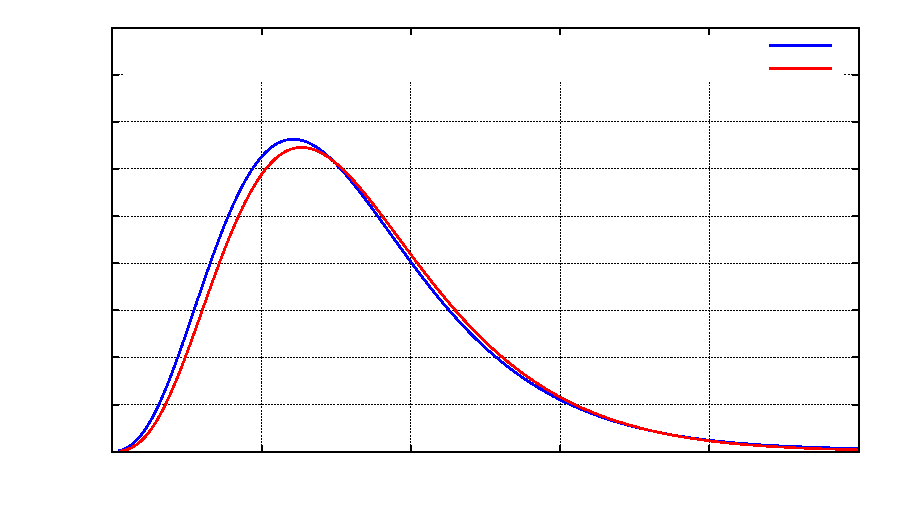
\includegraphics{graphs/gen}}%
    \gplfronttext
  \end{picture}%
\endgroup
}
  \caption{Histogram of $\log_{10}$ of absolute values of errors for solver generated by the systematical generator and for solver using the $F_4$ strategy.}
  \label{graph:gen}
\end{figure}

From the results, we can see that the numerical stability has remained the same for both solvers. The solver which uses the $F_4$ strategy is about 4 times faster than the~solver generated by the systematical polynomial generator.

\begin{landscape}
\begin{table}[ht]
  \centering
  \begin{tabular}{|c||ccc|}
    \hline
      & \textbf{One elimination} & \textbf{Multiple elimination} & \textbf{Multiple elimination} \\
      & \textbf{solver}          & \textbf{solver} ($step = 1$)  & \textbf{solver} ($step = 2$)\\
    \hline\hline
    \textbf{minimal} & 1.988 & 1.036 & 1.745\\
\textbf{median} & 2.799 & 2.003 & 2.198\\
\textbf{maximal} & 2.859 & 2.227 & 2.283\\

    \multirow{2}{*}{\textbf{sizes of matrices}} & \multirow{2}{*}{$185 \times 209$} & $64 \times 104; 80 \times 119$ & $133 \times 181$\\
                                                &                                   & $95 \times 125; 49 \times 73$  & $81 \times 105$\\
    \textbf{number of operations} & $9\;129\;329$ & $5\;152\;165$ & $7\;087\;366$\\
    \hline
  \end{tabular}
  \caption{Computing times of one and multiple elimination solvers.}
  \label{tab:elim}
\end{table}

\begin{table}[!ht]
  \centering
  \begin{tabular}{|c||ccc|}
    \hline
      & \textbf{Without matrix} & \textbf{Matrix partitioning}      & \textbf{Matrix paritioning} \\
      & \textbf{partitioning}   & \textbf{in the last elimination}  & \textbf{in all eliminations} \\
    \hline\hline
    \textbf{minimal time} & 1.353 s & 0.956 s & 0.794 s\\
\textbf{median of times} & 2.185 s & 1.071 s & 0.932 s\\
\textbf{maximal time} & 2.604 s & 1.189 s & 2.273 s\\

     \textbf{$1^{\text{st}}$ matrix} & $64 \times 104$ & $64 \times 104$                                      & $30 \times 47; 34 \times 44; 14 \times 35; 50\times 35$\\
     \textbf{$2^{\text{nd}}$ matrix} & $80 \times 119$ & $80 \times 119$                                      & $41 \times 48; 39 \times 49; 5 \times 29; 75 \times 29$\\
     \textbf{$3^{\text{rd}}$ matrix} & $95 \times 125$ & $95 \times 125$                                      & $50 \times 24; 45 \times 46; 32 \times 56; 63 \times 56$\\
     \textbf{$4^{\text{th}}$ matrix} & $49 \times 73$  & $29 \times 18;20 \times 15; 16 \times 40; 0\times 0$ & $29 \times 18;20 \times 15; 16 \times 40; 0\times 0$\\
     \textbf{number of operations} & $5\;152\;165$ & $4\;859\;537$ & $1\;775\;775$\\
    \hline
  \end{tabular}
  \caption{Computing times of solver without matrix partitioning, of solver with matrix partitioning in the last elimination only and of solver with matrix partitioning in all eliminations.}
  \label{tab:part}
\end{table}
\end{landscape}

~\vfill
\begin{table}[ht]
  \centering
  \begin{tabular}{|c||cc|}
    \hline
    & \textbf{Systematical}    & \textbf{$F_4$ strategy} \\
    &  \textbf{generator used} & \textbf{used} \\
    \hline\hline
    \textbf{minimal} & 2.213 & 0.615\\
\textbf{median} & 2.895 & 0.713\\
\textbf{maximal} & 3.320 & 1.161\\

    \multirow{6}{*}{\textbf{sizes of matrices}} & \multirow{6}{*}{$185 \times 209$} & $2 \times 12; 13 \times 30$\\
     & & $22\times46; 0\times 0$\\
     & & $52\times85; 36\times 65$\\
     & & $37\times62; 68\times 92$\\
     & & $44\times68; 0\times 0$\\
     & & $0\times0; 15\times 39$\\
     \textbf{number of operations} & $9\;129\;329$ & $2\;405\;581$\\
    \hline
  \end{tabular}
  \caption{Computing times of solver generated by the systematical generator and of the solver using the $F_4$ strategy.}
  \label{tab:gen}
\end{table}
\vfill
